\documentclass{article}
\usepackage[utf8]{inputenc}

\title{Software Design 2014 Final Report}
\author{Dimitar Dimitrov and Kyle Flores}
\date{May 2014}

\usepackage{graphicx}
\usepackage{placeins}

\begin{document}
\maketitle

\section*{Final Design Refinement}
\subsection*{Flow and Method}
%\FloatBarrier
\begin{figure}[ht!]
\centering
%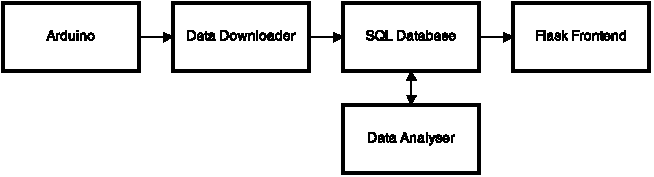
\includegraphics[width=5in]{flowpicture.png}
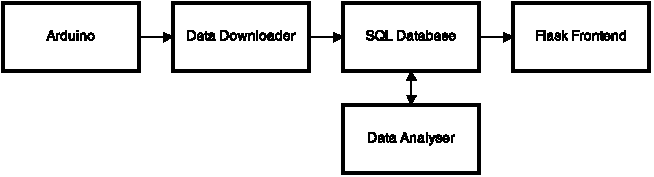
\includegraphics{flowpicture}
\caption{Graphical representation of the flow of information through our system.}
%\FloatBarrier
\end{figure}

\subsection*{Data Structures}
\par Most data was stored in SQLAlchemy objects.  While the program is running, active nodes are stored in lists.  Input data comes in the form of a dictionary.

\subsection*{UML Diagram}

\begin{figure}[ht!]
\centering
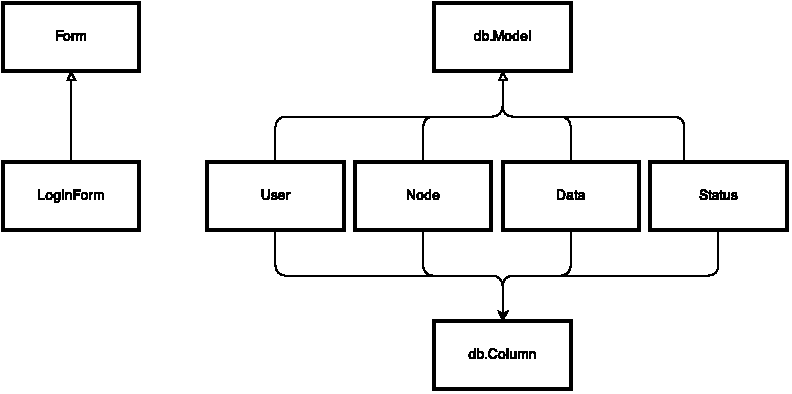
\includegraphics{UML}
\caption{UML diagram for SQL classes and Flask Login Manager}
\end{figure}

\section*{Results}
\par The product we presented during the class demo-day was something we were proud to put our names on. Because we reached our minimum deliverable relatively early in the project, our product incorporated some of the features we scoped out intially as extensions, and shows some refinement rtowards our design criteria
\begin{itemize}
 \item Detects when the door in a room is opened.
 \item Reports light and temperature values.
 \item Sensor kit servers secure a static IP address on the network.
 \item Data is stored to a SQLite database which is more certainly more robush than a csv.
 \item Flask integrates with SQLite and hosts a webapp on LAN that lets users view historical and current data
 \item Databases can be updated to accomodate new sensor nodes and sensor types without needing to reset the original databse.
 \item All configuration changes can be made without modifying source: Adding new sensor nodes requires modifying a "config.txt file" and migrating databases involves running a couple of python scripts.
\end{itemize}
Although in a software project, it is also possible to add more features, improve source maintainability, or beautify UI elements, we were satisfied with what we accomplished in the time alotted, considering also that we had a hardware component to work with, and learned to work with SQL and Flask independently.

\section*{Design Reflection}
\par We divided the system into very appropriate functinoal blocks, which made integration relatively easy.  We also ended up using very appropriate tools for each, namely Flask and SQLAlecemy.  Moving from CSV files to SQL for databasing was one of the best decisions we made.  In the future, however, we're thinking about changing the way communication works - namely having the Arduino's POST as opposed to the code GETing so that the system can be exported to an external server.

\section*{Division of Labor}
\par The first step of our project, networking hardware, was difficult to work on in parallel because all downstream elements depended on it. Until we had the Arduino sensor kits installed and network enabled, we could not write data acquisition scripts and it was difficult to determine how to create reasonable databases. We were able to write different aspects of the data acquistion routine in parallel however. The downloading from a webpage, webpage parsing, and data storage could be written independently provieded the input and output formats were known, which we did a decent job of documenting and keeping consistent. We later moved on to writing SQL models and the Flask app in parallel until the two were mature enough to be integrated. While this project was relatively large in scope for two people, our small team size ended up being appropriate.

\section*{Bugs and Future Extensions}
\par The worst kind of bugs are hardware bugs. We spent an absurd amount of time trying to figure out why our Arduino and ethernet controller would lose network connection at random times. After testing for Arduino C bugs, hardware connection issues, and ethernet port issues, we eventually discovered that the ENC28J60 breakout we were using was known to overheat on occasion due to poor board design. The problem was solved by taping a penny to the chip to help dissipate heat. 

\par Because neither of us had any experience with SQL prior to this project, SQLalchemy was at first unintuitive and tutorials were difficult to follow. Code we wrote to implement SQLite for our purposes was of course, difficult to debug too. Solutions were eventually found to most of the problems by iterative testing.

%\par Dimitar, you probably want to say something about Flask or web hosting here.

\section*{Acknowledgements and Closing Remarks}
Kyle and Dimitar would like to The Joshe and Aman for their advice and guidance the project, and Professor Paul Ruvolo for a great Software experience, and also for being a badass.

\end{document}
